% !TeX spellcheck = cs_CZ
{\tikzset{external/prefix={tikz/FYZI/}}
 \tikzset{external/figure name/.add={ch44_}{}}
%=========================== Kapitola: Zákony termodynamiky =======================================
\chapter{Zákony termodynamiky}\label{fyz:IchapXLIV}
\minitoc
  \section{Tepelné stroje; první zákon}\label{fyz:IchapXLIVsecI}
  \section{Druhý zákon}\label{fyz:IchapXLIVsecII}
  \section{Vratné stroje}\label{fyz:IchapXLIVsecIII}
  \section{Účinnost ideálního stroje}\label{fyz:IchapXLIVsecIV}
  \section{Termodynamická teplota}\label{fyz:IchapXLIVsecV}
  \section{Entropie}\label{fyz:IchapXLIVsecVI}
  \section{Příklady a cvičení}\label{fyz:IchapXLIVsecVII}

    \begin{figure}[ht!] %\ref{fyz_fig467}
      \centering
      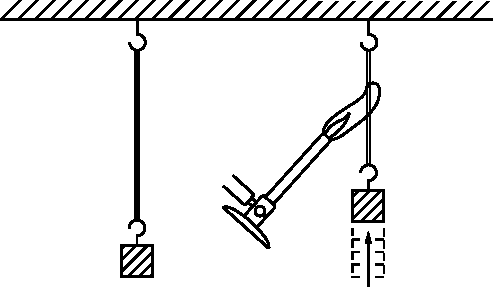
\includegraphics[width=0.7\linewidth]{fyz_fig467.pdf}
      \caption{ 
               (\cite[s.~707]{Feynman01})}
      \label{fyz_fig467}
    \end{figure}

    \begin{figure}[ht!] %\ref{fyz_fig468}
      \centering
      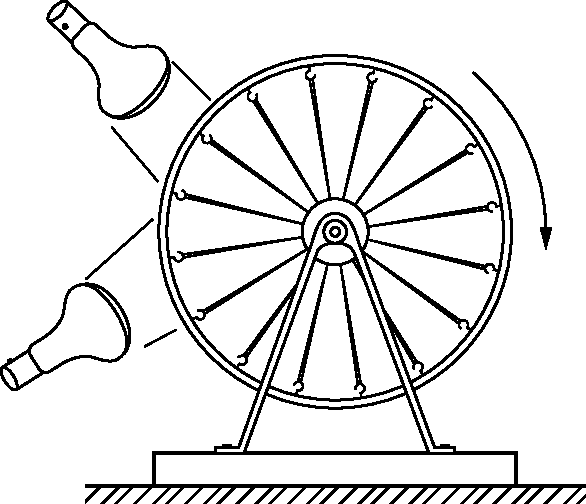
\includegraphics[width=0.7\linewidth]{fyz_fig468.pdf}
      \caption{ 
               (\cite[s.~707]{Feynman01})}
      \label{fyz_fig468}
    \end{figure}

    \begin{figure}[ht!] %\ref{fyz_fig469}
      \centering
      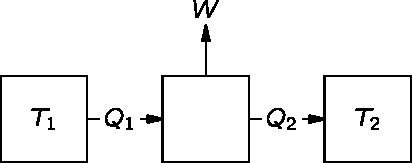
\includegraphics[width=0.7\linewidth]{fyz_fig469.pdf}
      \caption{ 
               (\cite[s.~707]{Feynman01})}
      \label{fyz_fig469}
    \end{figure}

    \begin{figure}[ht!] %\ref{fyz_fig470}
      \centering
      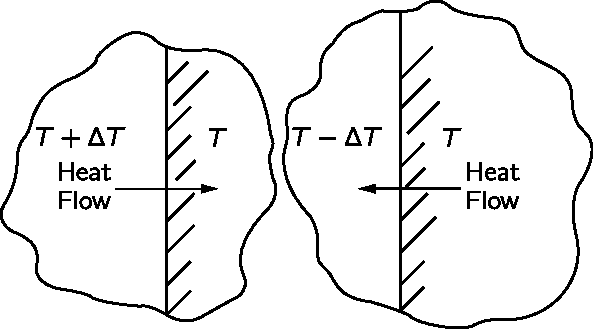
\includegraphics[width=0.7\linewidth]{fyz_fig470.pdf}
      \caption{ 
               (\cite[s.~707]{Feynman01})}
      \label{fyz_fig470}
    \end{figure}


  \begin{figure}[hb!] %\ref{fyz:fig471}
    \centering
    \begin{tabular}{c}
     \subfloat[ ]{\label{fyz:fig471a}
       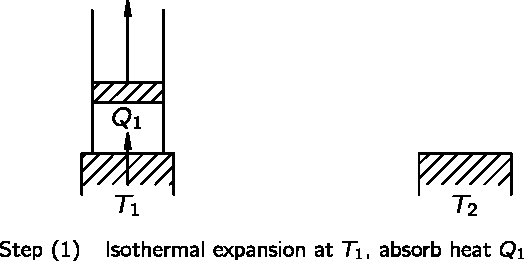
\includegraphics[width=0.7\linewidth]{fyz_fig471a.pdf}}  \\
     \subfloat[ ]{\label{fyz:fig471b}
       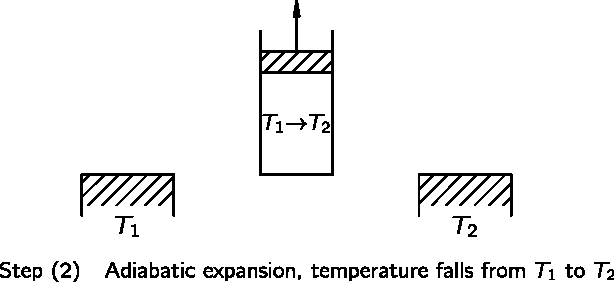
\includegraphics[width=0.7\linewidth]{fyz_fig471b.pdf}}  \\
     \subfloat[ ]{\label{fyz:fig471c}
       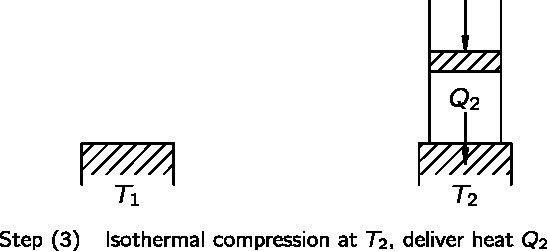
\includegraphics[width=0.7\linewidth]{fyz_fig471c.pdf}}  \\
     \subfloat[ ]{\label{fyz:fig471d}
       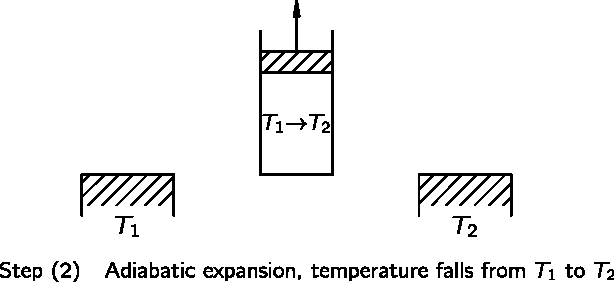
\includegraphics[width=0.7\linewidth]{fyz_fig471b.pdf}}  \\
    \end{tabular}
    \caption{
             (\cite[s.~601]{Feynman01}).}
    \label{fyz:fig471}
  \end{figure}

    \begin{figure}[ht!] %\ref{fyz_fig472}
      \centering
      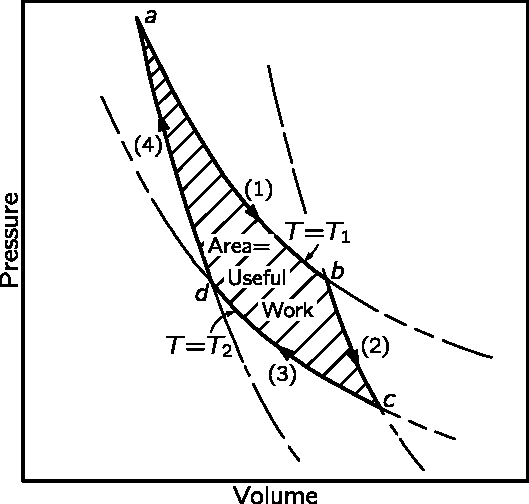
\includegraphics[width=0.7\linewidth]{fyz_fig472.pdf}
      \caption{ 
               (\cite[s.~707]{Feynman01})}
      \label{fyz_fig472}
    \end{figure}

    \begin{figure}[ht!] %\ref{fyz_fig473}
      \centering
      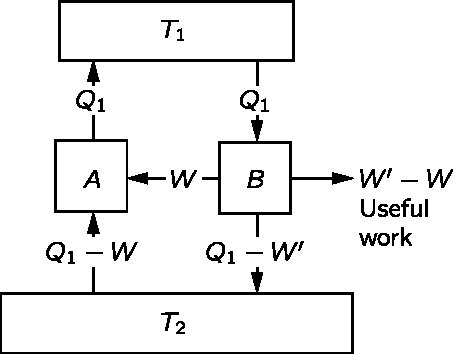
\includegraphics[width=0.7\linewidth]{fyz_fig473.pdf}
      \caption{ 
               (\cite[s.~707]{Feynman01})}
      \label{fyz_fig473}
    \end{figure}

    \begin{figure}[ht!] %\ref{fyz_fig474}
      \centering
      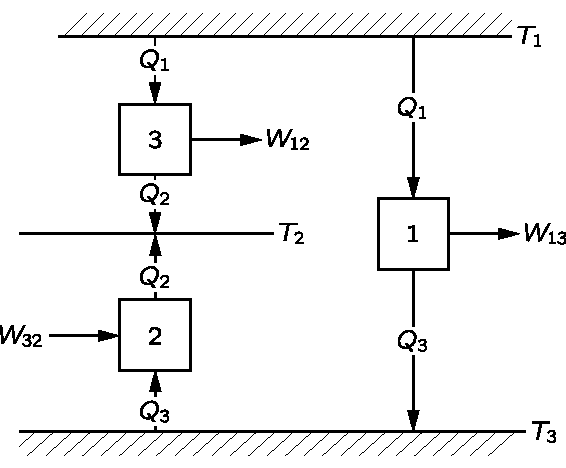
\includegraphics[width=0.7\linewidth]{fyz_fig474.pdf}
      \caption{ 
               (\cite[s.~707]{Feynman01})}
      \label{fyz_fig474}
    \end{figure}

    \begin{figure}[ht!] %\ref{fyz_fig475}
      \centering
      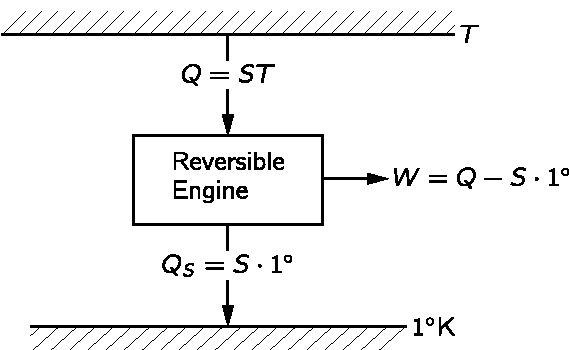
\includegraphics[width=0.7\linewidth]{fyz_fig475.pdf}
      \caption{ 
               (\cite[s.~707]{Feynman01})}
      \label{fyz_fig475}
    \end{figure}

    \begin{figure}[ht!] %\ref{fyz_fig476}
      \centering
      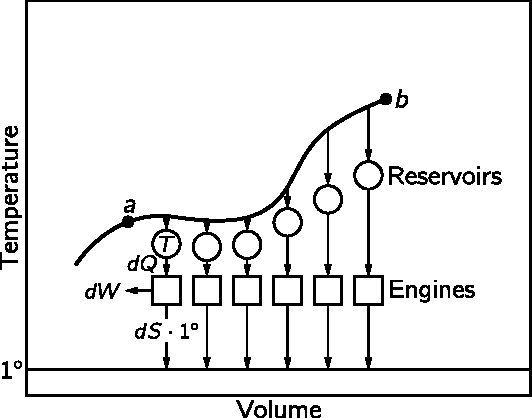
\includegraphics[width=0.7\linewidth]{fyz_fig476.pdf}
      \caption{ 
               (\cite[s.~707]{Feynman01})}
      \label{fyz_fig476}
    \end{figure}

    \begin{figure}[ht!] %\ref{fyz_fig477}
      \centering
      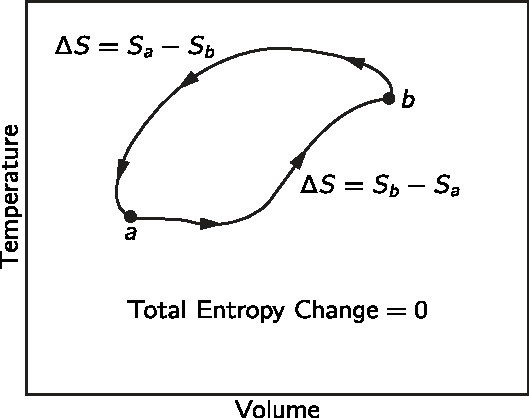
\includegraphics[width=0.7\linewidth]{fyz_fig477.pdf}
      \caption{ 
               (\cite[s.~707]{Feynman01})}
      \label{fyz_fig477}
    \end{figure}
  
} %tikzset
%---------------------------------------------------------------------------------------------------
\printbibliography[title={Seznam literatury}, heading=subbibliography]
\addcontentsline{toc}{section}{Seznam literatury}